% =====================================================================
% SS-RESfM — CVPR 2027 submission draft (ported from ICLR_ssresfm.tex Sep 6 2026)
% CVPR 2027: 8 pages INCLUDING figures/tables; references unlimited; double-blind.
% TODO before submission: replace cvpr.sty with the official CVPR 2027 Author Kit
% version and set the real Paper ID. [review] adds ruler + ID.
% Supplementary: CVPR_ssresfm_supp.tex (separate PDF).
% =====================================================================
\documentclass[10pt,twocolumn,letterpaper]{article}
\usepackage[review]{cvpr}
\usepackage{times}
\usepackage{graphicx,amsmath,amssymb,booktabs,multirow,xcolor}
\usepackage[pagebackref,breaklinks,colorlinks]{hyperref}
\def\confName{CVPR}
\def\confYear{2027}
\newcommand{\mad}{\textsc{madweight}}
\renewcommand{\deg}{^{\circ}}
\def\paperID{*****}
\title{When Outlier Supervision Fails:\\
Self-Supervised Robustness in Deep Structure-from-Motion}
\author{Anonymous CVPR submission\\ Paper ID *****}

\begin{document}
\maketitle
\begin{abstract}
To reconstruct cameras and 3D structure from real image collections, learning-based
Structure-from-Motion must reject \emph{outliers}: wrong correspondences that survive
geometric verification. The standard recipe trains an outlier classifier with labels
derived from an already-trusted reconstruction of the training scenes --- supervision
that presupposes exactly the capability it is meant to provide. We ask \emph{when this
recipe fails}, and show its failures are caused by the labels themselves, not by domain
shift: labels cannot be manufactured where robustness is needed most, and retraining the
state-of-the-art supervised method (RESfM) \emph{on} a $60\%$-contaminated domain with
best-case labels still loses $2\times$ to a label-free alternative. That alternative is
\textbf{SS-RESfM}: RESfM's outlier head trained with a \emph{self-supervised loss} ---
confident pseudo-labels formed from percentiles of the model's own reprojection error ---
with no ground-truth or COLMAP labels anywhere in training or test. Under a strictly controlled protocol (identical tracks, robust bundle adjustment,
and training schedule, varying only the outlier mechanism) we compare label-free
statistical removal (\mad{}) and soft reweighting against a from-scratch RESfM baseline
across six datasets spanning $0.5\%$--$61\%$ measured outliers. The optimal mechanism
\emph{flips with contamination}. Removal wins the high-contamination regime: at $61\%$
plain removal beats the supervised baseline on \emph{every} seed pair
($12.4\pm2.1$ vs.\ $19.2\pm3.4$) and both beat COLMAP, while at $43\%$ it beats every
supervised seed's median ($1.4$--$1.9$ vs.\ $2.4$--$4.3$). Reweighting wins the low-contamination regime, beating
the supervised baseline $2.5$--$2.9\times$ on two of the three clean out-of-distribution
splits (BlendedMVS and Olsson; Strecha goes to supervision on every seed) --- and,
unlike any supervised recipe we test, does so \emph{reliably}: the label-free arms land
in a narrow band on every training seed, whereas the supervised baseline collapses on
the clean benchmark in most seeds under every learning rate, budget, and recipe variant
we try (on Olsson --- $39$ essentially outlier-free scenes, $0.5\%$ --- every
MegaDepth-trained supervised variant lands at a translation error of $7.4$--$9.1$,
versus $2.9$--$3.6$ for every label-free arm). Supervision
retains the in-distribution regime and the cleanest OOD mean (self-supervised arms within
$\sim\!38\%$ in distribution). Every comparison is backed by five-training-seed bands, a
paired-seed evaluation control, and an environment-noise study --- in a benchmark family
where prior work fixes a single seed. We trace this to a structural circularity: outlier labels
require a trusted reconstruction of the very scenes whose contamination makes
reconstruction hard (for \emph{any} gold-standard labeler, not just COLMAP), and we
measure the resulting \emph{label ceiling}: regenerating supervision from scratch, label
recall collapses from $0.82$ to $\sim\!0.3$ above $\sim\!15\%$ contamination, precisely
where robustness is needed. Label-free adaptivity is thus a missing ingredient for robust
deep SfM.
\end{abstract}
\section{Introduction}
Structure-from-Motion (SfM) recovers camera poses and 3D structure from unordered image
collections. Its correspondences are heavily contaminated by outliers (wrong matches
that survive pairwise geometric verification), particularly in Internet photo collections
where repeated and symmetric structure produces spurious epipolar geometries. Classical
pipelines reject outliers with RANSAC and robust bundle adjustment (BA); recent deep
equivariant methods (ESFM~\citep{esfm}, RESfM~\citep{resfm}) instead learn a
\emph{sets-of-sets} permutation-equivariant network that regresses cameras from point
tracks and, in RESfM, adds a supervised per-point \emph{inlier/outlier classification
module}. RESfM's labels are derived from a COLMAP~\citep{colmap} reconstruction in two
stages: first by track membership, then refined by a $4$-pixel reprojection test against
COLMAP-pose triangulation~\citep{resfm}.

We take a different route. Rather than supervise the head with COLMAP labels, \textbf{SS-RESfM}
trains it \emph{self-supervised}: an adaptive confidence-weighted loss forms confident
pseudo-labels from percentiles of the model's own reprojection error, so no ground-truth or
COLMAP outlier labels are used anywhere in training or test. On top of this self-supervised
head we study a question RESfM's single supervised mechanism leaves open: \emph{is one
outlier-handling mechanism optimal across the range of contamination levels SfM encounters?}
We find that it is not. Holding everything else fixed and varying \emph{only} the
outlier-handling mechanism, the best mechanism \textbf{flips with contamination}:
hard removal at high contamination, soft reweighting at low, with the supervised
classifier retaining the typical in-distribution scene and the cleanest OOD mean
(Fig.~\ref{fig:complement}).
The removal family wins the high-contamination regime outright: plain removal beats
the supervised baseline on every seed at both $43\%$ and $\sim\!60\%$, while \mad{}
--- MAD-based removal with soft-weighted survivors, no learned threshold --- matches
the baseline there and beats COLMAP. The reason is structural, not incidental: outlier
labels must be derived from a trusted reconstruction of the very scenes whose
contamination makes reconstruction hard, so supervision bootstraps from precisely the
capability it is meant to provide --- and this circularity binds \emph{any}
gold-standard labeler, not just COLMAP. A self-supervised head consumes only the point
tracks; training data for robust SfM becomes as unlimited as unlabeled imagery, and new
domains need no labeling infrastructure.

\noindent\textbf{Contributions.}
(1)~\textbf{The label ceiling, measured and shown causal}: outlier supervision requires a
trusted reconstruction of the very scenes whose contamination makes reconstruction hard.
We measure the resulting label collapse (recall $0.82\!\to\!\sim\!0.3$ above
${\sim}15\%$ contamination) and prove it is causal, not domain shift: retrained
\emph{on} a $60\%$-contaminated domain with best-case labels, supervision still loses
$2\times$ to label-free removal (\S\ref{sec:indist}).
(2)~\textbf{The complementarity finding}: under an identical tracks+BA+schedule pipeline
isolating the mechanism alone, the optimal outlier mechanism flips with contamination ---
removal at high contamination (beating the supervised baseline on every seed pair at
$\sim\!60\%$), soft reweighting on clean OOD data ($2.5$--$2.9\times$, seed-reliably) ---
with supervision retaining a curated middle band.
(3)~\textbf{SS-RESfM}, the instrument of the study and a constructive answer: RESfM's
outlier handling made \emph{entirely} self-supervised via confident pseudo-labels from
the model's own reprojection-error percentiles --- no ground-truth or COLMAP labels
anywhere --- matching the supervised baseline where labels are sound and surpassing it
where they are not; plus \mad{}, which needs not even the head, removing by robust
reprojection statistics (MAD) and beating COLMAP where COLMAP's own labels cannot be
manufactured.
(4)~\textbf{A seed- and environment-level reliability methodology} for post-BA SfM
benchmarks: five-training-seed bands for every cell, a paired-seed evaluation control
($2{,}352$ evaluations showing the evaluation seed is immaterial), an
environment-noise floor for post-BA means, and per-seed-pairing claim verification ---
practices absent from this benchmark family, where prior work fixes a single seed, and
which surface findings (bimodal clean-OOD failures, basin-dependent escapes) that
mean$\pm$std alone would hide.
(5)~\textbf{A reusable robustness benchmark}: rebuilt Appendix-C-protocol track suites
for five OOD datasets with measured contamination ($0.5$--$61\%$), GT-derived outlier
labels, per-domain train/test splits, and the label-quality benchmark --- released with
code and configurations.

\section{Related Work}
\textbf{Deep equivariant SfM.} Learning-based SfM regresses cameras from point tracks with
permutation-equivariant networks. ESFM~\citep{esfm} casts uncalibrated SfM as deep projective
factorization over a measurement tensor, trained with an unsupervised reprojection loss;
GASFM~\citep{gasfm} uses a graph-attention variant. Both assume outliers were already removed
by two-view geometric verification. RESfM~\citep{resfm} targets contaminated internet
collections with a \emph{sets-of-sets} architecture plus a supervised per-point
inlier/outlier classification module and a robust BA, reporting accuracy close to its own
clean-track upper bound (``ESFM$^\ast$'') and on par with classical Theia/GLOMAP
(often with better translation recovery, while registering fewer images).
End-to-end pointmap and pose-regression pipelines (VGGSfM, MASt3R, DUSt3R) target far
smaller image sets. Concurrently, VGPA~\citep{vgpa} moved robustness to the
pose-averaging stage with a self-supervised relative-pose consistency objective ---
independently corroborating that label-free robustness is the frontier of deep SfM,
but at a different stage and input modality (pairwise relative poses vs.\ our
point-track matrices with per-observation outliers), so direct comparison is confounded.
We propose no new architecture: we reuse the RESfM/ESFM backbone and isolate the
outlier-handling stage and its supervision, with a reliability methodology that applies
to either paradigm.

\noindent\textbf{Outlier rejection, robust BA, and TTT.} Correspondence outliers that
\emph{survive} RANSAC/two-view filtering are the central difficulty in internet-scale
SfM; classical pipelines suppress them with M-estimators and robust BA, RESfM casts
rejection as supervised classification. We contrast that classification against
\emph{label-free} statistical removal via the median absolute deviation
(MAD)~\citep{mad} and soft reweighting, and show their relative merit is
contamination-dependent. RESfM's robust BA (outlier-point removal, largest connected
component, re-triangulation, re-optimization) is applied identically across all arms,
and per-scene test-time fine-tuning is treated as an orthogonal option ($\pm$TTT)
applied uniformly.

\section{Method}
\subsection{Background}
The input is a (sparse) point-track tensor $M$ of $m$ tracks across $n$ cameras, built by
concatenating pairwise RANSAC-verified SIFT matches. The sets-of-sets permutation-equivariant
network~\citep{resfm,esfm} maps $M$ to per-camera poses and a \emph{per-point} outlier score
$s\in[0,1]$ (points in the same track may receive different scores). Crucially, unlike RESfM,
whose classification head is trained with a BCE loss against \emph{COLMAP-derived}
inlier/outlier labels, SS-RESfM trains this head \emph{self-supervised}, with an adaptive
confidence-weighted loss: per forward pass it forms confident pseudo-labels from percentiles
of the model's own reprojection error (lowest $p$\% inliers, highest $p$\% outliers) and
applies BCE only to those. No ground-truth or COLMAP outlier labels are used at any point.
A reprojection error $e$ is available for every observation once an initial reconstruction
exists. All mechanisms below consume $s$ (and, for \mad{}, $e$),
produce a per-observation weight $w$ (or a hard keep/drop decision), and feed the result to
the identical robust-BA stage (Fig.~\ref{fig:method}).

\subsection{Outlier-handling mechanisms}
We compare four mechanisms, illustrated as weight-vs-signal transfer functions in
Fig.~\ref{fig:method}:
\begin{itemize}\itemsep2pt
\item\textbf{remove} (the RESfM analogue): drop a point if $s>\tau$; keep with $w{=}1$
otherwise. We use RESfM's default $\tau{=}0.6$ and its $\tau{=}0.8$ for the low-outlier,
single-camera Strecha/BlendedMVS sets~\citep{resfm}.
\item\textbf{weight}: soft, $w=1-s$, no removal.
\item\textbf{hybrid}: three-band: keep ($s$ below a low percentile), soft-weight (middle),
drop ($s$ above a high percentile).
\item\textbf{\mad{}} (ours): removal is driven by robust \emph{reprojection} statistics, not
the head. An observation is removed if its reprojection error exceeds
$\mathrm{med}(e)+\alpha\cdot\mathrm{MAD}(e)$ ($\alpha{=}2$); surviving observations are
soft-weighted by $w=1-s$. \mad{} is the only mechanism that consumes the reprojection
branch $e$ and requires \emph{no} learned threshold for removal.
\end{itemize}
Each mechanism is evaluated with and without test-time fine-tuning ($\pm$TTT), in which the
head continues to adapt on the test scene.

\subsection{Test-time fine-tuning and robust BA}
We load a multi-scene checkpoint, run a per-scene forward pass to obtain $s$ and $e$, apply
the mechanism, fine-tune per scene ($\sim\!1000$ iterations) under the reprojection
objective, and apply robust BA. This protocol, the seed, and the schedule are held fixed
across all arms; only the mechanism block changes.

\section{Experiments}
\subsection{Datasets and contamination}
We evaluate on six datasets spanning a wide contamination range. Alongside the RESfM
paper's quoted outlier fractions we report the contamination \emph{measured on our own
tracks} (robust ground-truth-pose triangulation with the standard $4$px cutoff, applied
uniformly to every dataset); see Table~\ref{tab:datasets}.
\begin{table}[t]\centering\footnotesize
\caption{\textbf{Datasets}: outlier rates (RESfM-reported vs.\ measured on our tracks) and regime.}
\label{tab:datasets}
\setlength{\tabcolsep}{1.2pt}%
\begin{tabular}{lccc}
\toprule
Dataset & RESfM\% & ours\% & Regime\\
\midrule
Strecha~\citep{strecha} & 2.7 & 1.7 & clean, LIDAR GT\\
BlendedMVS~\citep{blendedmvs} & 3.6 & 3.1 & low-outlier\\
MegaDepth~\citep{megadepth} & 25.6 & 25.4 & contam., \emph{in-dist.}\\
1DSfM~\citep{onedsfm} & 31.9 & 43.3 & contam., OOD\\
1DSfM-hard & -- & $\sim$60 & extreme, OOD\\
Olsson~\citep{olsson} & -- & 0.5 & outlier-free\\
\bottomrule
\end{tabular}
\end{table}
On MegaDepth (tracks identical to RESfM's) the two measurements agree ($25.4$ vs
$25.6$), validating the measurement; our 1DSfM rebuild ($43.3\%$) is markedly harder
than the tracks behind RESfM's quoted $31.9\%$. This yields a falsifiable prediction:
since the winning mechanism is a function of contamination (\S\ref{sec:indist}), on
the authors' own ${\sim}32\%$ 1DSfM tracks we expect supervision to be competitive or
ahead, with the label-free advantage emerging toward $43\%$ and dominating by $60\%$.
We state this in advance of evaluating on those tracks. \emph{1DSfM-hard} = the five
scenes unused by the standard ten-scene split, same pipeline, $300$ cameras per scene.
Networks train on 27 MegaDepth scenes; MegaDepth test is in-distribution, all other
datasets are OOD.

\subsection{Protocol, baselines, and track provenance}\label{sec:protocol}
Following RESfM's public code and default configuration, all networks train for
$20{,}000$ epochs (batch size, image subsampling, the eleven-milestone decay schedule,
and validation-based early stopping identical across arms), with five training seeds
($20$--$24$) per cell. Two deliberate settings are disclosed. First, the base learning
rate is per-method: $10^{-3}$ for the supervised arms (RESfM's released value),
$10^{-4}$ for the self-supervised arms, whose pseudo-label loss converges early (best
checkpoint ${\sim}$7.5k vs.\ ${\sim}$16.5k epochs); neither is truncation-limited.
Second, the infinity-point margin and the checkpoint-selection metric are held identical
across arms rather than at RESfM's released values --- a deviation that demonstrably
\emph{favors} the baseline: under the authors' own Accuracy-based selection it is
weaker on every dataset (RESfM-faithful row in Table~\ref{tab:main}; MegaDepth $0.50$
vs.\ $0.34$), so all supervised-baseline margins are lower bounds, and its
clean-benchmark failures persist under its own rule (Olsson $8.8$, BlendedMVS rotation
$53\deg$). We report shallow ($1{\times}3$) and deep ($2{\times}3$) architectures.

\noindent\textbf{Fair-comparison anchor.} Our controlled baseline is
\emph{RESfM-from-scratch}: trained by us with the \emph{identical} setup as our arms (same
27 scenes, sampling, epochs, seed), so only the outlier mechanism differs. We additionally
report \emph{RESfM-released} (authors' weights) and \emph{RESfM (paper)}.\footnote{The
ESFM row likewise follows the unified $20$k-epoch protocol. ESFM's own released
multi-scene (calibrated) recipe trains for $30$k epochs plus a $500$-epoch per-scene
fine-tune; we deliberately hold the schedule fixed across all rows so that the outlier
mechanism remains the only controlled variable.}

\noindent\textbf{Track provenance.} MegaDepth tracks and the 36 test scenes are
\emph{identical} to RESfM (directly comparable to published numbers). The OOD tracks
are \emph{built by us} from the released images and ground truth (RESfM did not release
OOD tracks), so OOD comparisons are controlled within our pipeline and \textbf{not}
directly comparable to RESfM's published OOD numbers. RESfM's released weights yield
$0.209$ on MegaDepth in our harness (vs.\ reported $0.169$; unchanged, $0.217$, under
the authors' exact pinned software stack), isolating the residual gap to solver-level
nondeterminism in robust BA (supplementary); the stack-replication study there shows
the no-TTT arms are insensitive to environment, while TTT \emph{means} inherit
solver-level noise.

\noindent\textbf{A method-isolated comparison, not a SOTA claim.}
RESfM-from-scratch shares every pipeline component with our arms and differs only in the
outlier mechanism --- the same controlled protocol RESfM uses when re-training
ESFM/GASFM in its pipeline. The anchor is also \emph{authors-faithful}: five retrains
under the authors' exact validation metric reproduce its five-seed band on every dataset
(supplementary), so the comparison does not depend on which supervised recipe one
prefers. We claim no SOTA: the \emph{released} checkpoint ($0.209$ on MegaDepth) beats
either from-scratch arm, but that gap stems from the released weights themselves (the
authors' own training code on our tracks reproduces $0.34$--$0.39$), handicapping
supervised and self-supervised arms \emph{equally}; RESfM-released and RESfM~(paper)
are reference rows throughout.

\noindent\textbf{Metrics.} Following RESfM we draw conclusions from post-BA
\emph{mean} errors (translation emphasized; rotation in degrees; translation is the
aligned camera-position error in scene coordinates), with medians as supporting
statistics --- except on 1DSfM, whose mean is dominated by two symmetric-structure
failure scenes (Ellis Island, Tower of London) that fail for \emph{all} methods; there
the median is representative. Rotation and registered-camera counts ($N_r$) for all
arms are tabulated in the supplementary; rotation broadly agrees with translation (the
supervised BlendedMVS failure is even larger in rotation), and under high contamination
the label-free arms register \emph{more} cameras than the supervised baseline
($38$--$43\%$ vs.\ $37\%$ on 1DSfM-hard). Two registration notions must be distinguished:
every learned arm outputs a pose for every camera (pose coverage; COLMAP genuinely fails
on $36\%$ of 1DSfM-hard), while $N_r$ counts the cameras surviving robust BA and a
$5$-pixel quality mask, the set over which errors are computed. Under this stricter
notion the plain-removal arms attain their low errors over a reduced set ($59\%$/$28\%$
vs.\ the baseline's $77\%$/$37\%$ on 1DSfM/1DSfM-hard), consistent with aggressive
pruning disconnecting weakly-supported cameras; \mad{} is registration-matched to the
baseline ($74\%$/$38\%$), so its comparisons are not coverage artifacts.

\begin{figure*}[t]
\centering
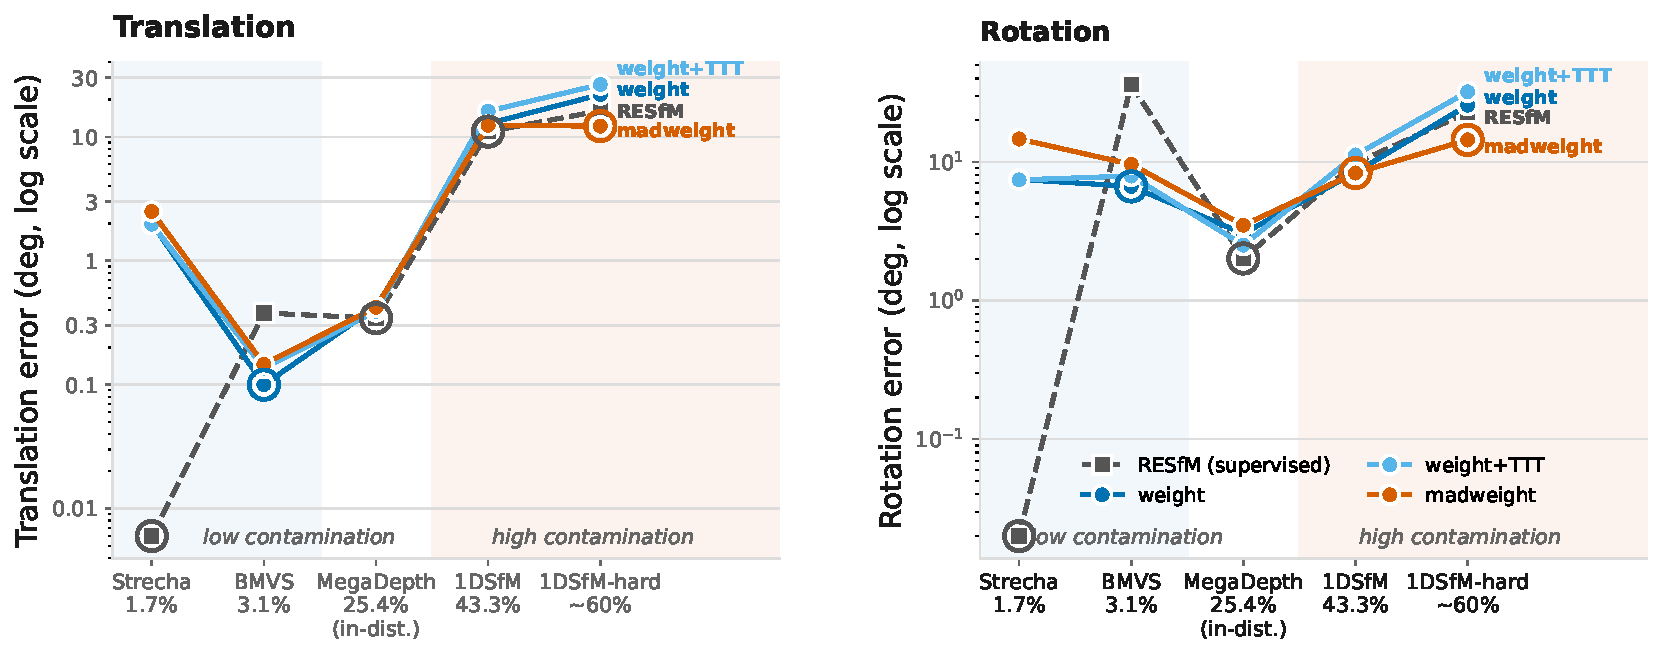
\includegraphics[width=0.76\textwidth]{PATHA_fig1_complementarity.pdf}
\caption{\textbf{The optimal outlier mechanism flips with contamination.} Translation
(left) and rotation (right) means (log scale) of the self-supervised arms vs.\ supervised
RESfM, five of the six datasets ordered by measured contamination
(Table~\ref{tab:main} data). Circled = best per dataset. The rotation panel mirrors the
translation ordering, with a self-supervised arm best on 1DSfM and the supervised
BlendedMVS failure even more pronounced ($36\deg$).}
\label{fig:complement}
\end{figure*}

\begin{figure*}[t]
\centering
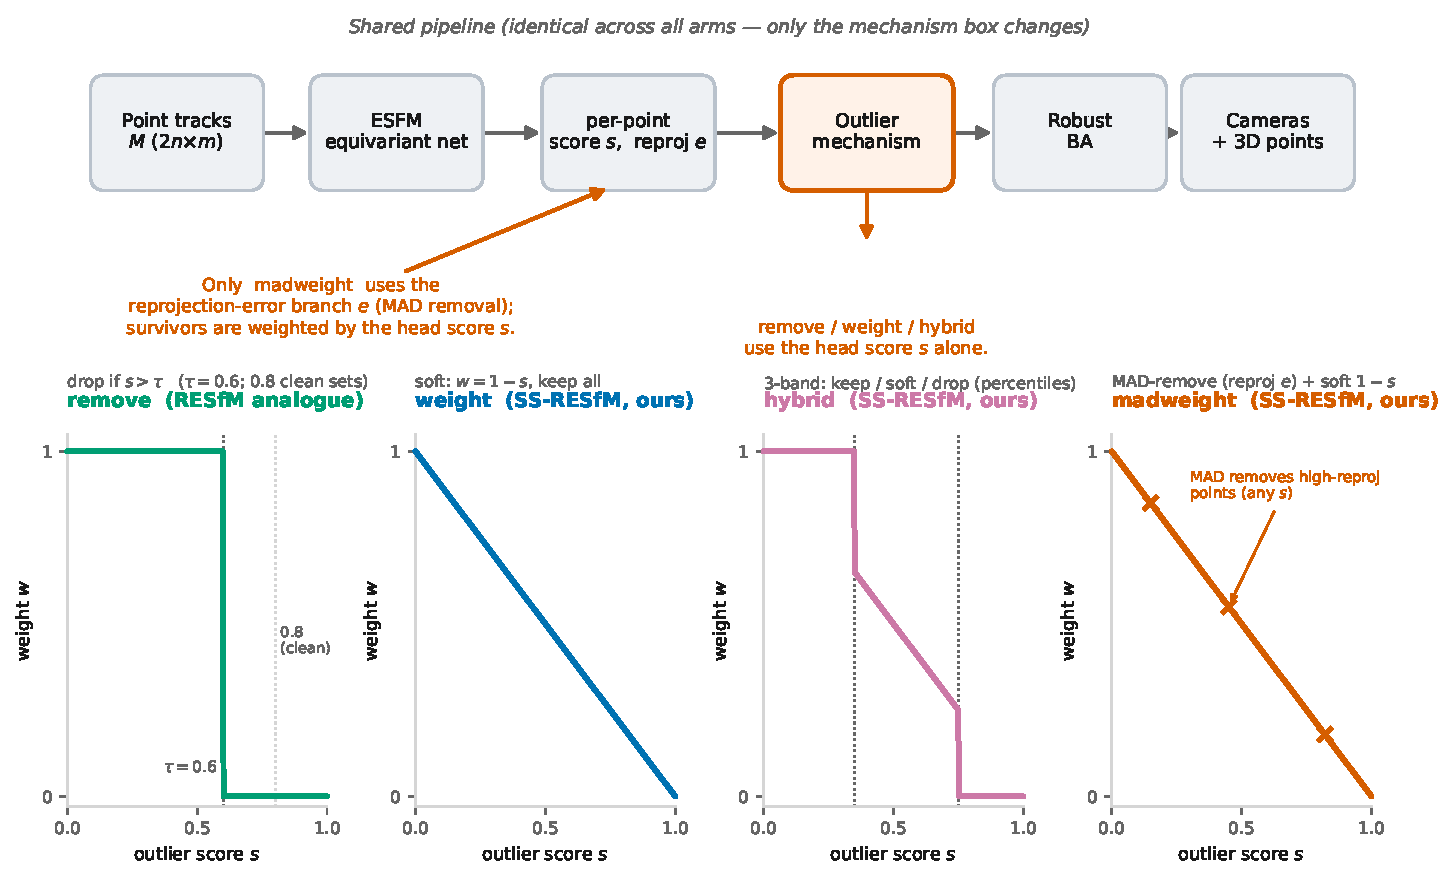
\includegraphics[width=0.7\textwidth]{PATHA_fig2_method.pdf}
\caption{\textbf{Method.} A shared pipeline (top) in which only the outlier-mechanism block
changes. The four mechanisms as weight-vs-signal transfer functions (bottom). Only \mad{}
consumes the reprojection-error branch $e$, and only for its removal step; its surviving
points are still weighted by the head score $s$ ($w{=}1{-}s$). The other three mechanisms
use $s$ alone.}
\label{fig:method}
\end{figure*}

\section{Results}
\subsection{Main comparison}
Table~\ref{tab:main} is the controlled head-to-head under the RESfM-aligned schedule:
every row shares tracks, architecture, schedule, robust BA, and seed, so any difference is
attributable to the outlier mechanism and its supervision alone. Reading along the
contamination axis:
(1)~\emph{Clean OOD} (Olsson $0.5\%$, Strecha $1.7\%$, BlendedMVS $3.1\%$): the
label-free arms win seed-robustly where the supervised head misfires: every arm beats
the full baseline band on BlendedMVS ($0.14$--$0.24$ vs.\ $0.35\pm0.04$; soft arms
$2.5\times$ better, and the baseline's $31.7\deg$ rotation failure persists on every
seed), and by ${\sim}3\times$ on Olsson against four of five baseline seeds
($3.0\pm0.3$ vs.\ $8.2$--$8.9$; one seed escapes at $2.69$ --- the collapse is
basin-dependent, frequency $4/5$). Figure~\ref{fig:qualolsson} shows what it looks
like: on an essentially outlier-free scene the supervised reconstruction degenerates to
a compressed cluster ($16.5\deg$ rotation), while the label-free arm reproduces the
ground-truth arc nearly exactly. Nor is the collapse a from-scratch artifact: the
released checkpoint also collapses on Olsson ($9.10$; $9.18$ under the authors' pinned
stack), as does the authors-faithful configuration ($8.77$). Strecha is the exception:
RESfM's mean wins on every seed ($0.006$--$1.67$ vs.\ $\sim\!2$), though the best
label-free median ties it ($0.005$) at seed 20.
(2)~\emph{In distribution} (MegaDepth), supervised RESfM retains mean and median.
Its mean is strongly seed-dependent ($0.37\pm0.12$ over five seeds; its best, $0.19$,
approaches the released checkpoint) while its median is stable ($0.07\pm0.02$); the
deterministic self-supervised arms band at $0.51\pm0.08$ and the TTT arm at
$0.40\pm0.11$ over five seeds; a $\sim\!38\%$ band-level gap without labels, not a win
(against the authors-faithful configuration, $0.496$, the arms reach parity, and the TTT
arm is ahead). Medians tell the same story more tightly ($0.13$--$0.20$ vs.\ $0.07$).
(3)~\emph{Moderate contamination} (1DSfM, $43\%$) has no stable winner between \mad{}
($11.0\pm1.7$) and the baseline ($10.5\pm1.5$; overlapping bands), so we decline a
directional claim for \mad{}. The \emph{removal family} leads on both statistics in
band terms: remove+TTT $8.9\pm1.2$ vs.\ the baseline's $10.5\pm1.5$ (separated means,
overlapping tails), and plain remove's medians ($1.7\pm0.2$) beat \emph{every} baseline
seed pairwise at five seeds each ($1.4$--$1.9$ vs.\ $2.4$--$4.3$; its means, $9.1\pm2.2$,
remain failure-scene-dominated): a label-free win at $43\%$ (the supplementary matrix table),
established against the baseline's own five-seed band.
(4)~\emph{Extreme contamination} (1DSfM-hard, ${\sim}60\%$): removal beats
weighting robustly, \mad{} ($18.9\pm4.1$) statistically matches the baseline
($19.2\pm3.4$), and plain remove goes further: $12.4\pm2.1$, below the baseline on
every one of the $25$ seed pairs (worst seed $15.8$ vs.\ the baseline's best $16.2$;
medians $10.8\pm2.8$ vs.\ $16.5\pm4.8$), and below the released checkpoint ($15.29$)
--- the extreme-contamination win holds against every supervised variant we can
construct or obtain, and all label-free arms are far ahead of COLMAP
(\S\ref{sec:extreme}). Rotation (Fig.~\ref{fig:complement}, right) follows the same
ordering. 

\begin{table*}[t]\centering\small
\caption{\textbf{Main controlled comparison (RESfM-aligned schedule).} Mean\,/\,median
post-BA translation error. All rows share tracks, architecture, schedule, robust BA, and
seeds; only the outlier mechanism and its supervision differ. Upper block = SS-RESfM arms
(five-training-seed bands, mean$\pm$std of per-seed dataset means), as is the supervised
baseline; reference and classical rows are single runs, except $^{\S}$RESfM~(released):
a band over five \emph{evaluation} seeds on the authors' fixed weights (network held
fixed, spread $\le\!0.008$ --- evaluation noise is negligible; training seeds are what
matter). Best per column in \textbf{bold}. ESFM$^{\ast}$ = vanilla ESFM on
ground-truth-cleaned tracks (clean-track reference; mean failure-scene-dominated, as in
RESfM's own Table~1).}
\label{tab:main}
\footnotesize\setlength{\tabcolsep}{3pt}%
\resizebox{\textwidth}{!}{%
\begin{tabular}{lcccccc}
\toprule
Arm & MegaDepth (25.4) & 1DSfM (43.3) & 1DSfM-hard (60) & Strecha (1.7) & BMVS (3.1) & Olsson (0.5)\\
 & $N_c{=}13126$ & $4563$ & $1497$ & $54$ & $225$ & $3858$\\
\midrule
\multicolumn{7}{l}{\emph{Translation error (mean\,/\,median), the primary metric}}\\[1pt]
\mad{}       & 0.51$\pm$0.08/0.16 & 11.0$\pm$1.7/4.9 & 18.9$\pm$4.1/13.4 & 2.65$\pm$0.25/1.16 & 0.14$\pm$0.02/0.05 & $\mathbf{3.0\pm 0.3}$/1.4\\
weight       & 0.51$\pm$0.09/0.20 & 14.4$\pm$3.0/9.6 & 22.9$\pm$2.8/15.6 & 1.97$\pm$0.09/0.04 & $\mathbf{0.14\pm 0.03}$/0.02 & 2.9$\pm$0.3/1.1\\
weight+TTT   & 0.40$\pm$0.11/0.18 & 15.7$\pm$2.1/10.8 & 22.2$\pm$3.2/15.3 & 2.00$\pm$0.05/0.12 & 0.14$\pm$0.02/$\mathbf{0.01}$ & 8.0$\pm$0.3/0.6\\
remove       & 0.51$\pm$0.08/0.13 & 9.1$\pm$2.2/$\mathbf{1.7\pm 0.2}$ & $\mathbf{12.4\pm 2.1}$/$\mathbf{10.8}$ & 3.20$\pm$0.11/2.03 & 0.24$\pm$0.06/0.17 & 3.4$\pm$0.6/1.7\\
remove+TTT   & 0.56$\pm$0.07/0.14 & $\mathbf{8.9\pm 1.2}$/2.0 & 15.2$\pm$1.0/11.3 & 3.01$\pm$0.07/1.70 & 0.22$\pm$0.10/0.18 & 3.6$\pm$0.4/1.9\\
RESfM-scratch (supervised)  & $\mathbf{0.37\pm 0.12}$/$\mathbf{0.07}$ & 10.5$\pm$1.5/3.4 & 19.2$\pm$3.4/16.5 & $\mathbf{0.39\pm 0.72}$/$\mathbf{0.01}$ & 0.35$\pm$0.04/0.33 & 7.4$\pm$2.6/$\mathbf{0.95}$\\
\midrule
RESfM (released)$^{\S}$    & 0.203$\pm$0.008 & 10.71$\pm$0.27 & 15.29 & 0.20$\pm$0.00 & 0.33$\pm$0.00 & 9.10\\
RESfM (paper)               & 0.169 & -- & -- & -- & -- & --\\
RESfM-faithful (authors' ckpt selection) & 0.496 & 9.75 & 17.58 & 0.144 & 0.367 & 8.77\\
ESFM$^{\ast}$ (clean tracks) & 0.60$\pm$0.18 & 13.24$\pm$0.52 & 18.12$\pm$4.35 & 1.14$\pm$0.45 & 3.79$\pm$3.51 & --\\
ESFM (same tracks, no outlier mech.) & 0.71$\pm$0.11 & 18.42$\pm$0.75 & 21.76$\pm$0.80 & 2.03$\pm$0.14 & 6.45$\pm$3.75 & 5.91$\pm$3.32\\
GASFM (released ckpt, our robust BA) & 2.25 & 25.84 & 36.49 & 1.14 & 11.13 & 4.45\\
GLOMAP (classical, global)  & 3.33 & 27.21 & 35.42 & $\mathbf{0.047}$ & 0.339 & 3.17\\
COLMAP (classical, increm.) & 0.62$\pm$0.03 & 6.29$\pm$0.42 & 20.4$\pm$1.1 & 0.03$\pm$0.00 & 0.01$\pm$0.00 & 0.20$\pm$0.00\\
\midrule
\bottomrule
\end{tabular}}
\end{table*}


\noindent\textbf{Classical baselines.} Running GLOMAP~(global) and COLMAP~(incremental)
on the \emph{same} tracks with known intrinsics reproduces the classical/deep trade-off
this literature reports, and sharpens it. GLOMAP is far the best method on pristine
calibrated data (Strecha $0.047$, an order of magnitude below every learned method;
Olsson median $0.087$) and registers almost everything ($96$--$100\%$ of cameras). Under
contamination its \emph{translations} collapse ($3.3$ on MegaDepth, $27.2$ at $43\%$,
$35.4$ at $60\%$, vs.\ $9.1$ and $12.4$ for label-free removal) while its
\emph{rotations} stay strong ($8.9\deg$ at $43\%$, better than the supervised
baseline's $9.6\deg$). The failure of classical global SfM under outlier contamination is
therefore specifically a positioning failure, not a loss of orientation structure, which
is also why translation is the metric of record in this setting. The comparison is not
compute- or coverage-matched: GLOMAP keeps $96\%$ of cameras at $43\%$ contamination
where plain removal keeps $58\%$, so the learned arms are far more accurate on a smaller
retained set.

\subsection{The complementarity finding}
Fig.~\ref{fig:complement} shows Table~\ref{tab:main} as a picture, and one pattern
organizes it. \emph{Between} supervision regimes, the self-supervised wins concentrate
exactly where a label-free design should help: on clean OOD data, where a classifier
trained on contaminated MegaDepth misfires (on BlendedMVS, RESfM's rotation error explodes
to $36\deg$), and at extreme contamination, where supervision itself can no longer be
manufactured (\S\ref{sec:whyremoval}). \emph{Within} the self-supervised family, the
removal-vs-weighting ordering is monotone in contamination: weighting is best at
$2$--$3\%$, the two tie in distribution, and removal dominates from $43\%$ upward
(\mad{} $12.4$ vs.\ weight $12.8$, plain remove $8.9$, the supplementary matrix table;
$12.4\pm2.1$ vs.\ $\sim\!23$ at $60\%$). This mechanism-level flip, the answer to our central
question, is stable across schedules and seeds.

\noindent\emph{Baseline learning-rate robustness, the full mechanism matrix, the
MAD/STD/Huber ablation, per-scene selection, and qualitative results are in the
supplementary.}

\begin{figure*}[t]\centering
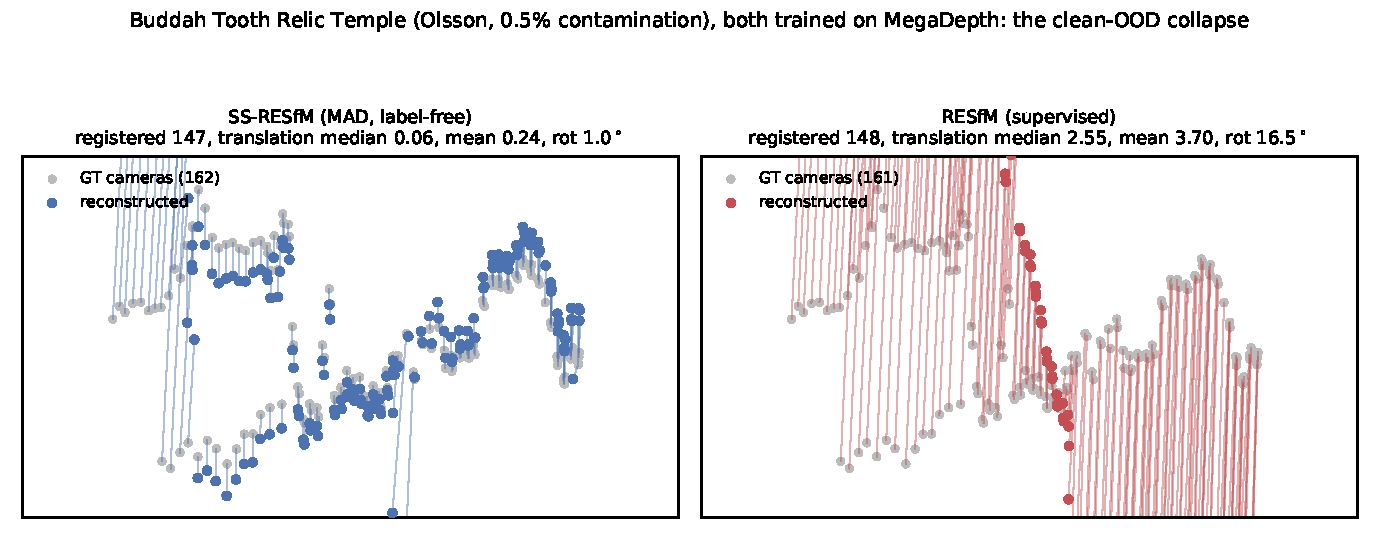
\includegraphics[width=0.74\textwidth]{fig_qual_olsson.pdf}
\caption{\textbf{The clean-OOD collapse, qualitatively} (Buddah Tooth Relic Temple,
Olsson, $0.5\%$ contamination; both networks trained on MegaDepth, seed $20$): top-view
camera centers in the evaluation frame; whiskers join each reconstructed camera to its
ground-truth position. The label-free \mad{} arm (left) lands on the ground-truth
layout (translation median $0.06$, rotation $1.0\deg$); the supervised baseline
(right) registers the same number of cameras but collapses them toward a line with
large systematic displacements (median $2.55$, rotation $16.5\deg$) --- on a scene
with almost no outliers to reject.}
\label{fig:qualolsson}
\end{figure*}

\subsection{Why label-free removal wins under high contamination}\label{sec:whyremoval}
Two factors explain the erosion of the supervised advantage. First, \emph{domain
shift}: the classifier's decision boundary, fit to MegaDepth, does not transfer to OOD
outlier statistics --- and even in distribution its classification is mediocre by
RESfM's \emph{own} ablation (outlier recall $72.1\%$ at precision $44.1\%$, their
Table~7), with their Appendix~D crediting much of the final accuracy to robust BA,
consistent with our pre/post-BA analysis (supplementary): much of the supervised
system's robustness is BA repair, not classification. Second, and more fundamentally,
the supervision itself degrades: RESfM's labeling assumes a COLMAP reconstruction and
ground-truth poses per training scene --- available for curated data, lacking exactly
where robustness is needed. \mad{} needs neither: it recomputes its outlier test
per-scene from reprojection statistics, so it is unaffected by domain shift wherever a
partial reconstruction exists.

\paragraph{Measuring the label ceiling.} We make the second argument quantitative:
on $18$ scenes spanning the contamination axis we regenerate labels as one must for a
\emph{new} dataset (from-scratch COLMAP on the same tracks, known intrinsics, no GT
poses) and score them against GT-pose reference labels (outlier = positive;
\emph{coverage} = fraction of observations receiving any verdict; $\le\!120$ cameras
per scene); Table~\ref{tab:ceiling}.
\begin{table}[t]\centering\footnotesize
\caption{\textbf{The label ceiling}: quality of COLMAP-regenerated supervision vs.\
contamination.}
\label{tab:ceiling}
\setlength{\tabcolsep}{3.5pt}%
\begin{tabular}{lccccc}
\toprule
Contam. & $n$ & Cover\% & Prec. & Recall & COLMAP $t$-err\\
\midrule
0--5\%    & 6 & 99.4 & 0.76 & 0.82 & 0.004\\
5--15\%   & 4 & 89.6 & 0.90 & 0.83 & 0.014\\
15--30\%  & 2 & 71.7 & 0.83 & $\mathbf{0.26}$ & 1.02\\
30--45\%  & 3 & 55.7 & 0.74 & $\mathbf{0.39}$ & 0.82\\
45--60\%  & 3 & 55.1 & 0.87 & $\mathbf{0.39}$ & 11.0\\
\bottomrule
\end{tabular}
\end{table}
Precision stays high throughout, but \emph{recall collapses} from $0.82$ to
$0.26$--$0.39$ and coverage halves once contamination exceeds ${\sim}15\%$: the corrupted
reconstruction absorbs enough outliers that most reproject acceptably under its distorted
geometry, and half the observations receive no label at all. A head trained on such labels
is actively taught that most true outliers are inliers, precisely where robustness
matters. Conversely, below ${\sim}15\%$ COLMAP-derived labels are excellent, consistent
with RESfM's strong in-distribution result and delimiting where the supervised recipe is
sound.

\subsection{Extreme contamination: the 1DSfM-hard set}\label{sec:extreme}
To probe beyond 1DSfM's $43\%$, we evaluate on the five held-out 1DSfM-hard scenes
($\sim\!60\%$ measured contamination, $300$ cameras each), adding COLMAP (incremental
mapping on the same tracks, known intrinsics) and the full mechanism grid
(supplementary table). The ordering extrapolates: over seeds
$20$--$24$, plain remove attains $12.4\pm2.1$ translation, below the supervised band
($19.2\pm3.4$) on \emph{every} seed pair (medians $10.8$ vs.\ $16.5$); \mad{}
($18.9\pm4.1$) statistically matches the baseline; every other mechanism (soft, hybrid,
alternative robust statistics) is at $16.9$ or worse at seed~20; and COLMAP loses
($20.9$) even though its error is computed \emph{only over the $64\%$ of cameras it
registers}. Errors are large for every method --- these scenes are hard --- but the
trend matches the label-ceiling prediction: the supervised advantage vanishes exactly
where supervision can no longer be manufactured. Strikingly, plain remove on the \emph{contaminated} tracks also beats
ESFM$^{\ast}$ on \emph{oracle-cleaned} tracks ($12.4\pm2.1$ vs.\ $18.12\pm4.35$;
$23$ of $25$ seed pairs): at $60\%$ contamination, even ground-truth labels used for
hard removal destroy more than they fix --- deleting $60\%$ of observations starves
tracks below the multi-view minimum and thins the viewing graph, whereas adaptive
removal with soft-weighted survivors preserves the constraint structure. Having
perfect labels would not rescue the removal-by-oracle recipe; the label ceiling is
thus not the only obstacle at the extreme --- \emph{how} labels are used matters as
much as having them.

\subsection{Training on the contaminated domains: the label ceiling is causal}\label{sec:indist}
The label-ceiling analysis predicts that supervision fails at high contamination because
the labels themselves become untrustworthy --- not because of domain shift. We test this
causally by making the OOD domains \emph{in-distribution}: for each dataset we split its
scenes into train/validation/held-out test and retrain both recipes on the domain itself
(identical protocol; supervised labels generated at reference quality, by the same
Appendix-C procedure as MegaDepth's but against each dataset's \emph{real} GT poses ---
the best case supervision could ever obtain). Table~\ref{tab:indist} reports five-seed
bands on the held-out scenes.

\begin{table*}[t]\centering\footnotesize
\setlength{\tabcolsep}{2pt}%
\caption{\textbf{In-distribution comparison on the (formerly OOD) domains}, ordered by
contamination: mean translation over held-out test scenes, mean$\pm$std over five
training seeds per recipe. Supervised labels are GT-derived (best case). Best per
column in \textbf{bold}.}
\label{tab:indist}
\setlength{\tabcolsep}{5pt}%
\begin{tabular}{lcccc}
\toprule
Arm & Olsson @$0.5\%$ & BlendedMVS @$3.1\%$ & 1DSfM @$43\%$ & 1DSfM-hard @$60\%$\\
\midrule
\mad{}      & 1.97$\pm$0.94 & 0.093$\pm$0.099 & 6.37$\pm$0.20 & $\mathbf{12.1\pm 6.1}$\\
weight      & 3.05$\pm$1.39 & 0.114$\pm$0.006 & 10.65$\pm$2.49 & 28.1$\pm$5.9\\
weight+TTT  & $\mathbf{1.60\pm 0.81}$ & $\mathbf{0.081\pm 0.046}$ & 9.91$\pm$2.39 & 29.3$\pm$8.4\\
remove      & 2.94$\pm$0.27 & 0.228$\pm$0.080 & 6.68$\pm$1.44 & 19.4$\pm$7.7\\
RESfM (sup., GT labels) & 2.03$\pm$1.86 & 0.260$\pm$0.149 & $\mathbf{4.97\pm 2.08}$ & 23.4$\pm$7.8\\
ESFM (no mechanism) & 1.45$\pm$1.44 & 2.36$\pm$3.27 & 10.20$\pm$2.97 & 23.14$\pm$5.89\\
\bottomrule
\end{tabular}
\end{table*}

\begin{figure*}[t]\centering
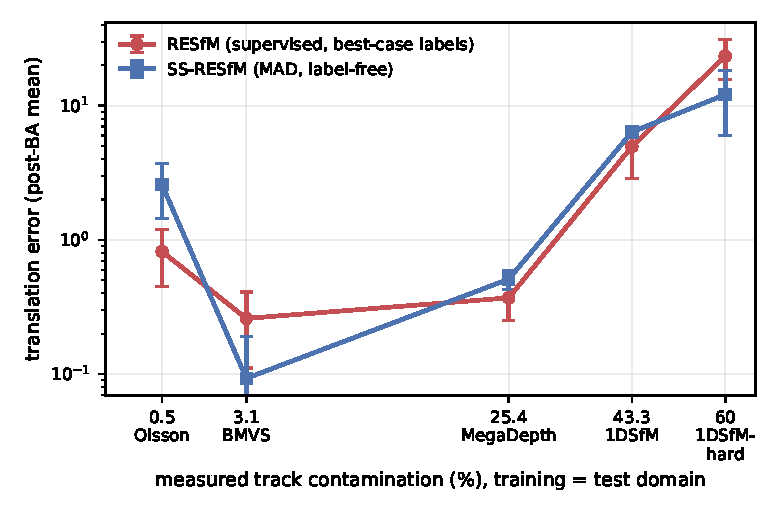
\includegraphics[width=0.72\textwidth]{fig_contamcurve.pdf}
\caption{\textbf{The completed in-distribution contamination curve.} Post-BA mean
translation (log scale) when training and test share the domain, versus measured track
contamination. The supervised recipe uses best-case labels (GT-derived; on MegaDepth,
its native COLMAP labels). Each label-free arm is its own line: soft weighting
($\pm$TTT) leads at low contamination, robust removal (\mad{}, remove) at high ---
the complementarity mechanism flip replicated in-distribution. Supervision
wins at $25\%$ and narrowly
at $43\%$, is seed-bimodal at $0.5\%$ (mean tied with the label-free arms at more than
twice their spread), and loses at $3.1\%$ (dataset-specific dead zone) and $60\%$ (the
causal label ceiling): its failures are two distinct modes, not a smooth function of
contamination. The rotation panel (right) tells the same story and makes the BlendedMVS
dead zone starker still (supervised $20.7\pm12.2\deg$ vs.\ label-free $4$--$13\deg$).
Bands: $\pm$std over five training seeds (MegaDepth rotation: five-seed means, bands
omitted).}
\label{fig:contamcurve}
\end{figure*}

Four findings (Fig.~\ref{fig:contamcurve}). \emph{(i) At $60\%$, supervision loses on its own training domain}: the
supervised head, trained on these scenes with reference-quality labels, is beaten
$\sim\!2\times$ at band level by \mad{} ($12.1\pm6.1$ vs.\ $23.4\pm7.8$; four of five
\mad{} seeds beat every supervised seed; medians $9.8$ vs.\ $20.6$). ``Just train the
classifier there'' does not work: the high-contamination failure is caused by labeling at
contamination, not by domain shift. Sharper still: the supervised head with best-case labels performs
\emph{identically to no outlier mechanism at all} at this contamination (vanilla ESFM
trained in-domain: $23.14\pm5.89$ vs.\ supervised $23.4\pm7.8$) --- at $60\%$,
GT-supervised classification adds nothing over doing nothing, while label-free removal
halves both. The vanilla row completes a symmetric statement: GT-label supervision
matches \emph{no mechanism at all} at both extremes of the axis --- identical at
$60\%$ ($23.4$ vs.\ $23.1$) and overlapping at $0.5\%$ in-domain ($2.03\pm1.86$
vs.\ $1.45\pm1.44$) --- earning its keep only in the curated middle band
($25$--$43\%$). The absolute errors deserve decomposition (supplementary figure): they are
not uniformly ``large for everyone.'' On Roman\_Forum, \mad{} produces \emph{usable}
reconstructions (median $1.6$--$3.5$, rotation $2.3$--$8.2\deg$, in four of five seeds)
where supervision fails outright (medians $9.5$--$36$); on Union\_Square the supervised
errors look lower but are computed over only $43$--$55$ of $300$ registered cameras,
versus \mad{}'s $137$--$186$ --- the error-vs-coverage trade-off of
\S\ref{sec:protocol} again, with the label-free arm covering $3$--$4\times$ more of
the scene at moderate error. \emph{(ii) The BlendedMVS failure was never domain
shift either}: supervision trained \emph{on} BlendedMVS lands at $0.20$--$0.37$ in four
of five seeds --- indistinguishable from the MegaDepth-trained baseline evaluated OOD
($0.35\pm0.04$) --- with a single escape seed ($0.02$), the same bimodality as its
clean-OOD behaviour, while label-free weighting is seed-stable at $0.114\pm0.006$.
Class imbalance alone cannot explain this: at $0.5\%$ (Olsson), where positives are
rarer still, supervision trained in-domain reaches $0.41$--$1.08$ in three of five
seeds --- extreme positive scarcity does not preclude learning --- whereas BlendedMVS
never reaches that level on any seed; the BlendedMVS failure is a dataset-specific
dead zone (its rotation pathology is the leading suspect), not a general
low-contamination bound. \emph{(iii) In-domain training attenuates but does not cure
the clean-benchmark unreliability}: the recipe that lands at $7.4$--$9.1$ on Olsson
MegaDepth-trained improves to $2.03\pm1.86$ trained in-domain --- but bimodally,
excellent in three seeds ($0.41$--$1.08$) and degraded in two ($3.9$--$4.2$, rotation
spread $12\pm12\deg$). The OOD collapse is thus mostly the MegaDepth-fit head
misclassifying on clean scenes (in-domain labels remove the bulk of it), yet the
seed-reliability asymmetry survives even here: weight+TTT ($1.60\pm0.81$) leads the
column, \mad{} ($1.97\pm0.94$) matches the supervised mean at half the spread, and no
label-free arm has a failure seed. Supervision's clean-data advantage is a
three-in-five-seeds advantage, not a dependable one. \emph{(iv) The supervised
advantage inverts between $43\%$ and $60\%$} ($4.97\pm2.08$ vs.\ \mad{}
$6.37\pm0.20$ at $43\%$; a $2\times$ loss at $60\%$), and the complementarity
ordering replicates in-distribution --- the mechanism flip is a property of the
contamination level, not the train/test relationship. Read as a curve, best-case-label supervision wins at $25\%$ and narrowly $43\%$, is
seed-bimodal at $0.5\%$ (tied in mean, far wider in spread), and loses at $3.1\%$ and
$60\%$: two distinct failure modes --- a dataset-specific dead zone, and the causal
label ceiling that no in-domain retraining can cross --- with seed-unreliability
shadowing the whole axis.


\section{Limitations}
(1)~No single deployable configuration wins all datasets; selecting the best mechanism per
dataset (Table~\ref{tab:main}) requires knowing the contamination level. We present a study
of the phenomenon, not a turnkey adaptive method; an unsupervised selector is future work. Relatedly, the basin-dependent character of the clean-OOD failures
(\S\ref{sec:indist}; the reliability appendix) suggests a natural remedy we do not
pursue here: initializing or anchoring the joint reconstruction with \emph{label-free
global pose averaging} (cf.\ the concurrent view-graph work of~\citealt{vgpa}), which
would compose two self-supervised robustness mechanisms at complementary stages of the
pipeline --- graph-level pose consistency selecting the basin, track-level adaptivity
handling observations --- toward a fully self-supervised robust SfM pipeline. We leave
this composition to future work.
(2)~Supervised RESfM retains in-distribution MegaDepth (the self-supervised arms come
within $\sim\!38\%$ at the band level, no closer) and the clean Strecha mean, and RESfM-released
remains stronger on MegaDepth, so we claim no SOTA. (3)~\mad{} matches rather than beats supervision at moderate/extreme contamination;
plain remove leads every baseline seed pairwise at $\sim\!60\%$ and on medians at
$43\%$, but over a reduced registered set (\S\ref{sec:protocol}), and the
\emph{magnitude} of the supervised deficit at BlendedMVS and high contamination is
learning-rate-dependent (supplementary) --- the Olsson collapse and the mechanism flip
are not. (4)~OOD tracks are self-constructed (not comparable to RESfM's published OOD
numbers). (5)~Two symmetric-structure scenes fail for all methods --- the cases where
excess removal disconnects the viewing graph~\citep{resfm}.

\section{Conclusion}
SS-RESfM makes deep SfM outlier handling \emph{entirely self-supervised} while staying
within $\sim\!38\%$ of the supervised baseline in distribution, winning two of three
clean-OOD splits --- reliably, on every training seed --- and beating it at high
contamination on every seed pair, where both beat COLMAP and supervision itself can no
longer be manufactured. The optimal mechanism is contamination-dependent: removal at
high contamination, reweighting at low. Robust deep SfM should treat outlier handling as
adaptive and self-supervised; code, configurations, and the rebuilt OOD tracks will be
released upon publication.

\label{sec:endcontent}%
\begin{thebibliography}{99}\small

\bibitem[Khatib et al.(2025)]{resfm} Khatib, Kasten, Moran, Galun, and Basri. RESfM: Robust Deep Equivariant Structure from Motion. ICLR 2025.

\bibitem[Moran et al.(2021)]{esfm} Moran, Koslowsky, Kasten, Maron, Galun, and Basri. Deep Permutation Equivariant Structure from Motion. ICCV 2021.

\bibitem[Brynte et al.(2024)]{gasfm} Brynte, Iglesias, Olsson, and Kahl. Learning Structure-from-Motion with Graph Attention Networks. CVPR 2024.

\bibitem[Sch\"onberger and Frahm(2016)]{colmap} Sch\"onberger and Frahm. Structure-from-Motion Revisited. CVPR 2016.

\bibitem[Rousseeuw and Croux(1993)]{mad} Rousseeuw and Croux. Alternatives to the Median Absolute Deviation. JASA 1993.

\bibitem[Wilson and Snavely(2014)]{onedsfm} Wilson and Snavely. Robust Global Translations with 1DSfM. ECCV 2014.

\bibitem[Li and Snavely(2018)]{megadepth} Li and Snavely. MegaDepth: Learning Single-View Depth Prediction from Internet Photos. CVPR 2018.

\bibitem[Strecha et al.(2008)]{strecha} Strecha, von Hansen, Van Gool, Fua, and Thoennessen. On Benchmarking Camera Calibration and Multi-View Stereo for High-Resolution Imagery. CVPR 2008.

\bibitem[Yao et al.(2020)]{blendedmvs} Yao et al. BlendedMVS: A Large-Scale Dataset for Generalized Multi-View Stereo Networks. CVPR 2020.

\bibitem[Khatib et al.(2026)]{vgpa} Khatib, Galun, and Basri. Learning Global Camera Poses from Noisy View-Graphs for Structure from Motion (VGPA). ECCV 2026.

\bibitem[Olsson and Enqvist(2011)]{olsson} Olsson and Enqvist. Stable Structure from Motion for Unordered Image Collections. SCIA 2011.

\end{thebibliography}


\end{document}
